\documentclass[ignorenonframetext,]{beamer}
\setbeamertemplate{caption}[numbered]
\setbeamertemplate{caption label separator}{: }
\setbeamercolor{caption name}{fg=normal text.fg}
\beamertemplatenavigationsymbolsempty
\usepackage{lmodern}
\usepackage{amssymb,amsmath}
\usepackage{ifxetex,ifluatex}
\usepackage{fixltx2e} % provides \textsubscript
\ifnum 0\ifxetex 1\fi\ifluatex 1\fi=0 % if pdftex
\usepackage[T1]{fontenc}
\usepackage[utf8]{inputenc}
\else % if luatex or xelatex
\ifxetex
\usepackage{mathspec}
\else
\usepackage{fontspec}
\fi
\defaultfontfeatures{Ligatures=TeX,Scale=MatchLowercase}
\fi
% use upquote if available, for straight quotes in verbatim environments
\IfFileExists{upquote.sty}{\usepackage{upquote}}{}
% use microtype if available
\IfFileExists{microtype.sty}{%
\usepackage{microtype}
\UseMicrotypeSet[protrusion]{basicmath} % disable protrusion for tt fonts
}{}
\newif\ifbibliography
\usepackage{color}
\usepackage{fancyvrb}
\newcommand{\VerbBar}{|}
\newcommand{\VERB}{\Verb[commandchars=\\\{\}]}
\DefineVerbatimEnvironment{Highlighting}{Verbatim}{commandchars=\\\{\}}
% Add ',fontsize=\small' for more characters per line
\usepackage{framed}
\definecolor{shadecolor}{RGB}{248,248,248}
\newenvironment{Shaded}{\begin{snugshade}}{\end{snugshade}}
\newcommand{\KeywordTok}[1]{\textcolor[rgb]{0.13,0.29,0.53}{\textbf{{#1}}}}
\newcommand{\DataTypeTok}[1]{\textcolor[rgb]{0.13,0.29,0.53}{{#1}}}
\newcommand{\DecValTok}[1]{\textcolor[rgb]{0.00,0.00,0.81}{{#1}}}
\newcommand{\BaseNTok}[1]{\textcolor[rgb]{0.00,0.00,0.81}{{#1}}}
\newcommand{\FloatTok}[1]{\textcolor[rgb]{0.00,0.00,0.81}{{#1}}}
\newcommand{\ConstantTok}[1]{\textcolor[rgb]{0.00,0.00,0.00}{{#1}}}
\newcommand{\CharTok}[1]{\textcolor[rgb]{0.31,0.60,0.02}{{#1}}}
\newcommand{\SpecialCharTok}[1]{\textcolor[rgb]{0.00,0.00,0.00}{{#1}}}
\newcommand{\StringTok}[1]{\textcolor[rgb]{0.31,0.60,0.02}{{#1}}}
\newcommand{\VerbatimStringTok}[1]{\textcolor[rgb]{0.31,0.60,0.02}{{#1}}}
\newcommand{\SpecialStringTok}[1]{\textcolor[rgb]{0.31,0.60,0.02}{{#1}}}
\newcommand{\ImportTok}[1]{{#1}}
\newcommand{\CommentTok}[1]{\textcolor[rgb]{0.56,0.35,0.01}{\textit{{#1}}}}
\newcommand{\DocumentationTok}[1]{\textcolor[rgb]{0.56,0.35,0.01}{\textbf{\textit{{#1}}}}}
\newcommand{\AnnotationTok}[1]{\textcolor[rgb]{0.56,0.35,0.01}{\textbf{\textit{{#1}}}}}
\newcommand{\CommentVarTok}[1]{\textcolor[rgb]{0.56,0.35,0.01}{\textbf{\textit{{#1}}}}}
\newcommand{\OtherTok}[1]{\textcolor[rgb]{0.56,0.35,0.01}{{#1}}}
\newcommand{\FunctionTok}[1]{\textcolor[rgb]{0.00,0.00,0.00}{{#1}}}
\newcommand{\VariableTok}[1]{\textcolor[rgb]{0.00,0.00,0.00}{{#1}}}
\newcommand{\ControlFlowTok}[1]{\textcolor[rgb]{0.13,0.29,0.53}{\textbf{{#1}}}}
\newcommand{\OperatorTok}[1]{\textcolor[rgb]{0.81,0.36,0.00}{\textbf{{#1}}}}
\newcommand{\BuiltInTok}[1]{{#1}}
\newcommand{\ExtensionTok}[1]{{#1}}
\newcommand{\PreprocessorTok}[1]{\textcolor[rgb]{0.56,0.35,0.01}{\textit{{#1}}}}
\newcommand{\AttributeTok}[1]{\textcolor[rgb]{0.77,0.63,0.00}{{#1}}}
\newcommand{\RegionMarkerTok}[1]{{#1}}
\newcommand{\InformationTok}[1]{\textcolor[rgb]{0.56,0.35,0.01}{\textbf{\textit{{#1}}}}}
\newcommand{\WarningTok}[1]{\textcolor[rgb]{0.56,0.35,0.01}{\textbf{\textit{{#1}}}}}
\newcommand{\AlertTok}[1]{\textcolor[rgb]{0.94,0.16,0.16}{{#1}}}
\newcommand{\ErrorTok}[1]{\textcolor[rgb]{0.64,0.00,0.00}{\textbf{{#1}}}}
\newcommand{\NormalTok}[1]{{#1}}
\usepackage{graphicx,grffile}
\makeatletter
\def\maxwidth{\ifdim\Gin@nat@width>\linewidth\linewidth\else\Gin@nat@width\fi}
\def\maxheight{\ifdim\Gin@nat@height>\textheight0.8\textheight\else\Gin@nat@height\fi}
\makeatother
% Scale images if necessary, so that they will not overflow the page
% margins by default, and it is still possible to overwrite the defaults
% using explicit options in \includegraphics[width, height, ...]{}
\setkeys{Gin}{width=\maxwidth,height=\maxheight,keepaspectratio}

% Prevent slide breaks in the middle of a paragraph:
\widowpenalties 1 10000
\raggedbottom

\AtBeginPart{
\let\insertpartnumber\relax
\let\partname\relax
\frame{\partpage}
}
\AtBeginSection{
\ifbibliography
\else
\let\insertsectionnumber\relax
\let\sectionname\relax
\frame{\sectionpage}
\fi
}
\AtBeginSubsection{
\let\insertsubsectionnumber\relax
\let\subsectionname\relax
\frame{\subsectionpage}
}

\setlength{\parindent}{0pt}
\setlength{\parskip}{6pt plus 2pt minus 1pt}
\setlength{\emergencystretch}{3em}  % prevent overfull lines
\providecommand{\tightlist}{%
\setlength{\itemsep}{0pt}\setlength{\parskip}{0pt}}
\setcounter{secnumdepth}{0}
\setbeamertemplate{itemize items}[ball]
\hypersetup{colorlinks,urlcolor=blue}
\addtobeamertemplate{headline}{\hypersetup{linkcolor=.}}{}
\addtobeamertemplate{footline}{\hypersetup{linkcolor=.}}{}
\usepackage{graphicx}

\title{MFE Programming Workshop}
\subtitle{Interfacing R to Other Languages}
\author{Brett Dunn}
\date{Fall 2016}

\begin{document}
\frame{\titlepage}

\begin{frame}{Why would you want to use another language?}

\begin{itemize}
\tightlist
\item
  R is great, but it has some weaknesses

  \begin{itemize}
  \tightlist
  \item
    For example, loops can be slow
  \end{itemize}
\item
  It is sometimes desirable to call code written in other languages from
  R.
\item
  Also, you may want to call R from a another language
\item
  R interfaces have been developed for a number of other languages

  \begin{itemize}
  \tightlist
  \item
    We will focus on C/C++
  \end{itemize}
\item
  The main motivation in performance enhancement

  \begin{itemize}
  \tightlist
  \item
    C/C++ code may run much faster than R
  \end{itemize}
\end{itemize}

\end{frame}

\begin{frame}[fragile]{Writing C/C++ Functions to be called from R}

\begin{itemize}
\tightlist
\item
  Key points to remember:

  \begin{itemize}
  \tightlist
  \item
    All the argurments passedd from R to C/C++ are received by C/C++ as
    pointers
  \item
    The C/C++ function itself must return \texttt{void}

    \begin{itemize}
    \tightlist
    \item
      Hence, we need to pass a pointer for the result
    \end{itemize}
  \item
    For R to work with C++ code (or even C code compiled with g++), you
    need to wrap your functions inside an an extern statement: extern
    ``C'' \{ yourC++\_code\_here\ldots{}. \} (or just declare with
    extern statement)
  \end{itemize}
\item
  We will learn to compile code using R (via gcc and g++) and Visual
  C++.
\item
  The end product is a dynamic shared library file (.so) on Linux/OS X
  or a dynamic-link library

  \begin{itemize}
  \tightlist
  \item
    DLLs are a common way to incorporate number-crunching C++ code in a
    front-end like R or Excel.
  \end{itemize}
\end{itemize}

\end{frame}

\begin{frame}{Required software}

\begin{itemize}
\tightlist
\item
  On windows, you need to install Rtools, available
  \href{https://cran.r-project.org/bin/windows/Rtools/}{here}

  \begin{itemize}
  \tightlist
  \item
    Just choose the version that matches your computer architecture
    (i.e.~64 bit or 32 bit)
  \item
    You have the make sure Rtools is in you path (may need to restart)
  \end{itemize}
\item
  Please verify:

  \begin{itemize}
  \tightlist
  \item
    On Linux you need to have GNU gcc and g++ (probably already
    installed)

    \begin{itemize}
    \tightlist
    \item
      Do you need r-base-dev?
    \end{itemize}
  \item
    On OS X, you may need Xcode.
  \end{itemize}
\end{itemize}

\end{frame}

\begin{frame}[fragile]{Our program: \texttt{timesTwo.cpp}}

\Large

\begin{Shaded}
\begin{Highlighting}[]
\DataTypeTok{extern} \StringTok{"C"} \DataTypeTok{void}
  \NormalTok{timesTwo(}\DataTypeTok{double} \NormalTok{*in, }\DataTypeTok{double} \NormalTok{*out)}
\NormalTok{\{}
  \DataTypeTok{double} \NormalTok{value = in[}\DecValTok{0}\NormalTok{] * }\FloatTok{2.0}\NormalTok{;}
    \NormalTok{out[}\DecValTok{0}\NormalTok{] = value;}
\NormalTok{\}}
\end{Highlighting}
\end{Shaded}

\end{frame}

\begin{frame}[fragile]{What does \texttt{extern\ "C"} do?}

\begin{itemize}
\tightlist
\item
  Remember R is written in C.
\item
  \texttt{extern\ "C"} makes our C++ function available to a program
  written in C (i.e.~R).

  \begin{itemize}
  \tightlist
  \item
    It declares the functions with C linkage
  \item
    If we write a C program, we don't need it
  \end{itemize}
\item
  Note that the parameter and return types are constained.

  \begin{itemize}
  \tightlist
  \item
    For example, cannot write a function that passes a (nontrivial) C++
    class to a C program
  \item
    The C program would not know what to do about the contructors,
    destructors, and other class-specific operations.
  \end{itemize}

\begin{Shaded}
\begin{Highlighting}[]
\DataTypeTok{extern} \StringTok{"C"} \DataTypeTok{void}
  \NormalTok{timesTwo(}\DataTypeTok{double} \NormalTok{*in, }\DataTypeTok{double} \NormalTok{*out)}
\NormalTok{\{}
  \DataTypeTok{double} \NormalTok{value = in[}\DecValTok{0}\NormalTok{] * }\FloatTok{2.0}\NormalTok{;}
    \NormalTok{out[}\DecValTok{0}\NormalTok{] = value;}
\NormalTok{\}}
\end{Highlighting}
\end{Shaded}
\end{itemize}

\end{frame}

\begin{frame}[fragile]{Compile using R's command line tools}

\begin{itemize}
\tightlist
\item
  In R, you can type:
\end{itemize}

\begin{Shaded}
\begin{Highlighting}[]
\KeywordTok{system}\NormalTok{(}\StringTok{"R CMD SHLIB timesTwo.cpp"}\NormalTok{)}
\end{Highlighting}
\end{Shaded}

\begin{itemize}
\tightlist
\item
  Or, on the command line:
\end{itemize}

\centerline{
  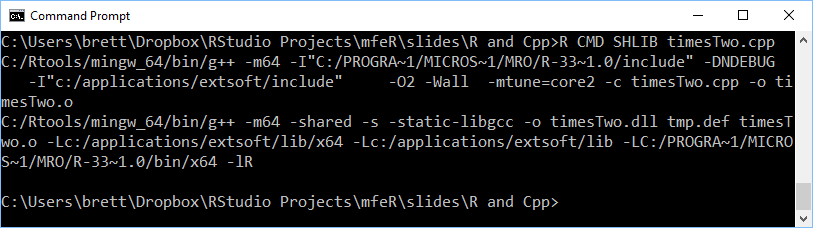
\includegraphics[width=\textwidth,height=0.4\textheight,keepaspectratio]{./RcmdSHLIB}
}

\begin{itemize}
\tightlist
\item
  Now we have timesTwo.dll (or timesTwo.so) ready to use in R
\end{itemize}

\end{frame}

\begin{frame}[fragile]{Now run the DLL in R}

\begin{Shaded}
\begin{Highlighting}[]
\KeywordTok{dyn.load}\NormalTok{(}\StringTok{"./timesTwo.dll"}\NormalTok{)}
\NormalTok{value_in <-}\StringTok{ }\DecValTok{32}\NormalTok{; value_out <-}\StringTok{ }\DecValTok{0}
\KeywordTok{.C}\NormalTok{(}\StringTok{"timesTwo"}\NormalTok{, }\KeywordTok{as.double}\NormalTok{(value_in), }
   \DataTypeTok{res=}\KeywordTok{as.double}\NormalTok{(value_out))$res}
\end{Highlighting}
\end{Shaded}

\begin{verbatim}
## [1] 64
\end{verbatim}

\begin{Shaded}
\begin{Highlighting}[]
\KeywordTok{dyn.unload}\NormalTok{(}\StringTok{"./timesTwo.dll"}\NormalTok{)}
\end{Highlighting}
\end{Shaded}

\begin{itemize}
\tightlist
\item
  \texttt{dyn.load} loads the .dll into R
\item
  \texttt{.C} calls timesTwo, and passes value\_in and value\_out to the
  function

  \begin{itemize}
  \tightlist
  \item
    \texttt{.C} returns a list, so we define `result' and extract
    `result' from the list
  \end{itemize}
\item
  \texttt{dyn.unload} unloads the .dll from R (you need the unload the
  dll if you want to rebuild it).
\end{itemize}

\end{frame}

\begin{frame}{Creating a DLL project in Visual Studio 2015}

\begin{itemize}
\tightlist
\item
  Choose File/New/Project../Win32 Project
\end{itemize}

\centerline{
  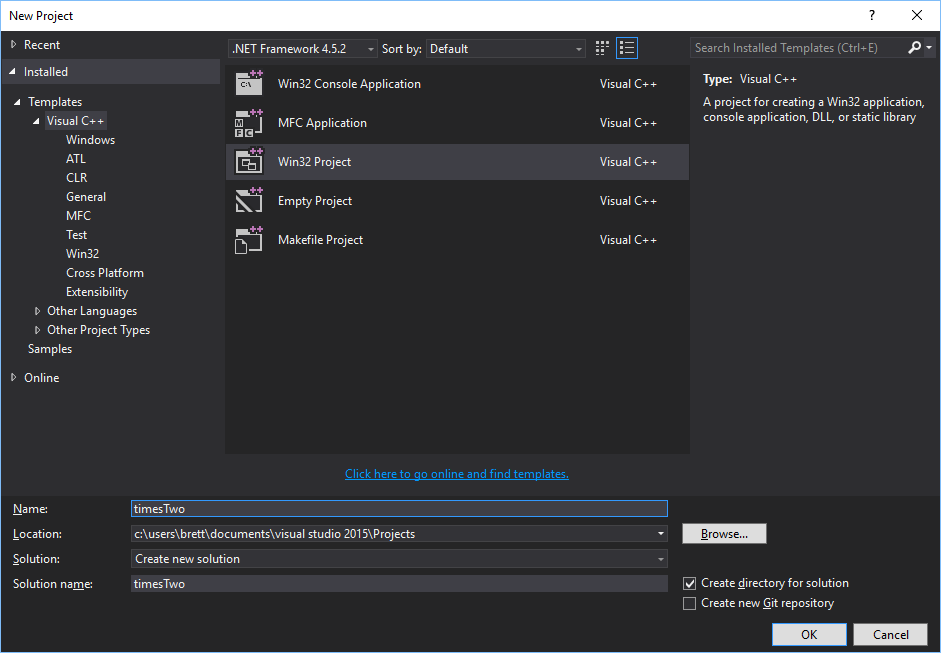
\includegraphics[width=\textwidth,height=0.7\textheight,keepaspectratio]{./project.png}
}

\end{frame}

\begin{frame}{Creating a DLL project in Visual Studio 2015}

\begin{itemize}
\tightlist
\item
  Specify a DLL and an Empty project
\end{itemize}

\centerline{
  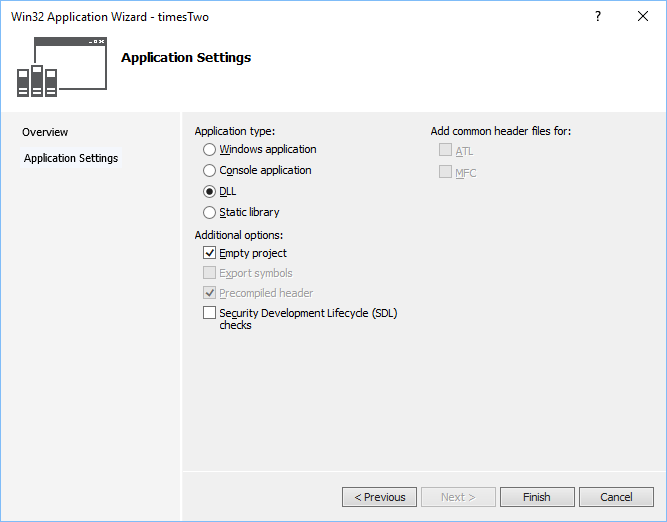
\includegraphics[width=\textwidth,height=0.7\textheight,keepaspectratio]{./settings.png}
}

\end{frame}

\begin{frame}{Project at This Point}

\centerline{
  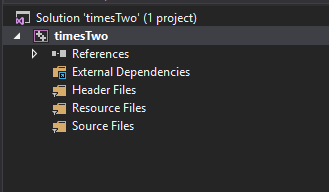
\includegraphics[width=\textwidth,height=0.7\textheight,keepaspectratio]{./projectToPoint}
}

\end{frame}

\begin{frame}{Add a C++ Source File}

-Right-click Source Files in the Solution Explorer, then select Add New
Item, and then select C++ File (.cpp)

\centerline{
  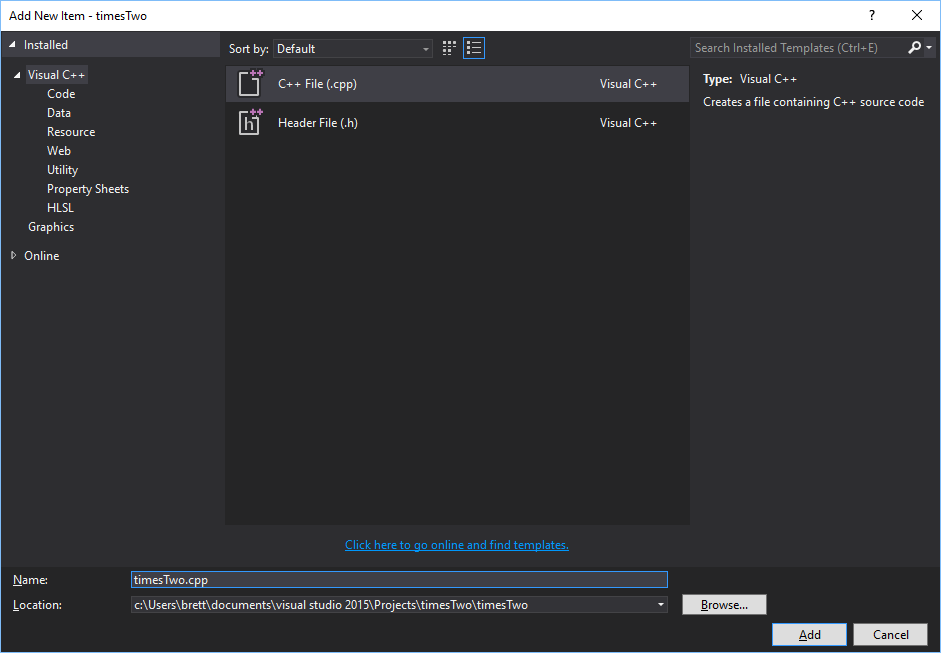
\includegraphics[width=\textwidth,height=0.7\textheight,keepaspectratio]{./addNewItem}
}

\end{frame}

\begin{frame}[fragile]{Add C++ Code to the Source File}

\LARGE

\begin{Shaded}
\begin{Highlighting}[]
\DataTypeTok{extern} \StringTok{"C"} \DataTypeTok{void} \NormalTok{__cdecl }
  \NormalTok{timesTwo(}\DataTypeTok{double} \NormalTok{*in, }\DataTypeTok{double} \NormalTok{*out)}
\NormalTok{\{}
  \DataTypeTok{double} \NormalTok{value = in[}\DecValTok{0}\NormalTok{] * }\FloatTok{2.0}\NormalTok{;}
    \NormalTok{out[}\DecValTok{0}\NormalTok{] = value;}
\NormalTok{\}}
\end{Highlighting}
\end{Shaded}

\end{frame}

\begin{frame}[fragile]{What is \texttt{\_\_cdecl} about?}

\begin{itemize}
\tightlist
\item
  Applies only to Windows.
\item
  The Visual C++ compilers allow you to specify conventions for passing
  arguments and return values between functions and callers.
\item
  Two options we care about:

  \begin{itemize}
  \tightlist
  \item
    \textbf{\texttt{\_\_cdecl}} is used by C/C++ programs, R, Matlab,
    SAS, others.
  \item
    \textbf{\texttt{\_\_stdcall}} is used by Excel, Win32 API fuctions,
    Pascal, others.
  \end{itemize}
\item
  This all essentially amounts to conventions for who (function caller
  or function) pops arguments off the stack.
\item
  For more information, see
  \href{https://msdn.microsoft.com/en-us/library/984x0h58.aspx}{this
  webpage}.
\end{itemize}

\begin{Shaded}
\begin{Highlighting}[]
\DataTypeTok{extern} \StringTok{"C"} \DataTypeTok{void} \NormalTok{__cdecl }
  \NormalTok{timesTwo(}\DataTypeTok{double} \NormalTok{*in, }\DataTypeTok{double} \NormalTok{*out)}
\NormalTok{\{}
  \DataTypeTok{double} \NormalTok{value = in[}\DecValTok{0}\NormalTok{] * }\FloatTok{2.0}\NormalTok{;}
  \NormalTok{out[}\DecValTok{0}\NormalTok{] = value;}
\NormalTok{\}}
\end{Highlighting}
\end{Shaded}

\end{frame}

\begin{frame}[fragile]{Why are we using pointers?}

\begin{itemize}
\tightlist
\item
  In C++ \texttt{timesTwo(double\&\ in,\ double\&\ out)} works as well
\end{itemize}

\begin{Shaded}
\begin{Highlighting}[]
\DataTypeTok{extern} \StringTok{"C"} \DataTypeTok{void} \NormalTok{__cdecl }
  \NormalTok{timesTwo(}\DataTypeTok{double} \NormalTok{*in, }\DataTypeTok{double} \NormalTok{*out)}
\NormalTok{\{}
  \DataTypeTok{double} \NormalTok{value = in[}\DecValTok{0}\NormalTok{] * }\FloatTok{2.0}\NormalTok{;}
  \NormalTok{out[}\DecValTok{0}\NormalTok{] = value;}
\NormalTok{\}}
\end{Highlighting}
\end{Shaded}

\end{frame}

\begin{frame}{Add a Module Definition File (.def)}

\begin{itemize}
\tightlist
\item
  Add New Item\ldots{}Under Visual C++ / Code you will find the .def
  file.
\end{itemize}

\centerline{
  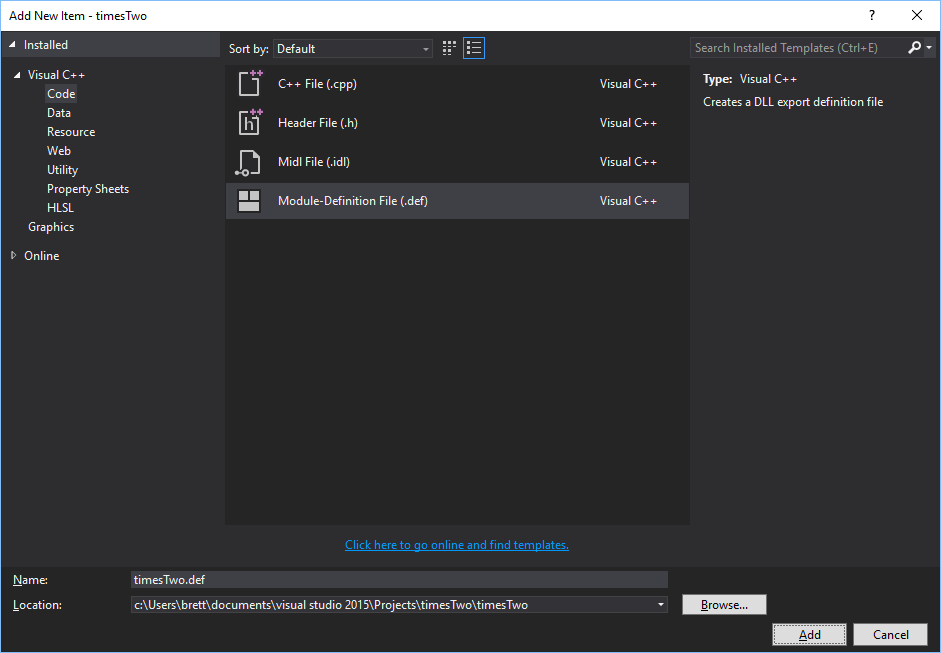
\includegraphics[width=\textwidth,height=0.7\textheight,keepaspectratio]{./defFile.png}
}

\end{frame}

\begin{frame}[fragile]{Module Definition File}

\begin{itemize}
\tightlist
\item
  A .def file is a module definition file. This is a convenient way to
  tell the linker which parts of our C++ code we want to export.
\end{itemize}

\begin{Shaded}
\begin{Highlighting}[]
\CommentTok{// timesTwo.def}
\NormalTok{LIBRARY timesTwoDLL}
\NormalTok{EXPORTS}
  \NormalTok{timesTwo}
\end{Highlighting}
\end{Shaded}

\begin{itemize}
\tightlist
\item
  \texttt{LIBRARY} is the name of the DLL
\item
  \texttt{EXPORTS} lists the functions to be exported (each one on a
  seprate line)

  \begin{itemize}
  \tightlist
  \item
    If you want to use a different function name use
    \texttt{newName\ =\ oldName}
  \end{itemize}
\end{itemize}

\end{frame}

\begin{frame}[fragile]{Another option: \texttt{\_\_declspec(dllexport)}}

\begin{itemize}
\tightlist
\item
  Windows-specific.
\item
  On Windows, we need to tell which functions are exported from the DLL.

  \begin{itemize}
  \tightlist
  \item
    That is, which funtions will be available in R.
  \end{itemize}
\item
  we
\item
  When building your DLL, you typically create a header file that
  contains the functions you are exporting and add
  \texttt{\_\_declspec(dllexport)} to the declarations in the header
  file.
\item
  For more information, see
  \href{https://msdn.microsoft.com/en-us/library/a90k134d.aspx}{this.}
\item
  Instead of \texttt{\_\_declspec(dllexport)}, you can use a
  \href{https://msdn.microsoft.com/en-us/library/d91k01sh.aspx}{DEF
  file.}
\end{itemize}

\end{frame}

\begin{frame}{Build the Solution}

\begin{itemize}
\tightlist
\item
  Make sure to change the architecture to x64 before building (unless
  you are using 32bit R) 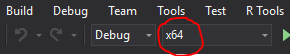
\includegraphics{./x64.PNG}
\item
  Ctrl-Shift-B builds the solution.
\item
  The DLL is found in the ./x64/Debug folder 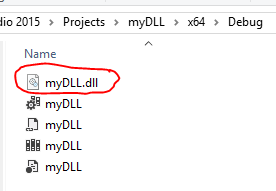
\includegraphics{./DLL.PNG}
\end{itemize}

\end{frame}

\begin{frame}{Add an R project to Visual Studio}

\begin{itemize}
\tightlist
\item
  Right click the solution\ldots{}Add\ldots{}New Project\ldots{}Other
  Languages\ldots{}R project
\end{itemize}

\centerline{
  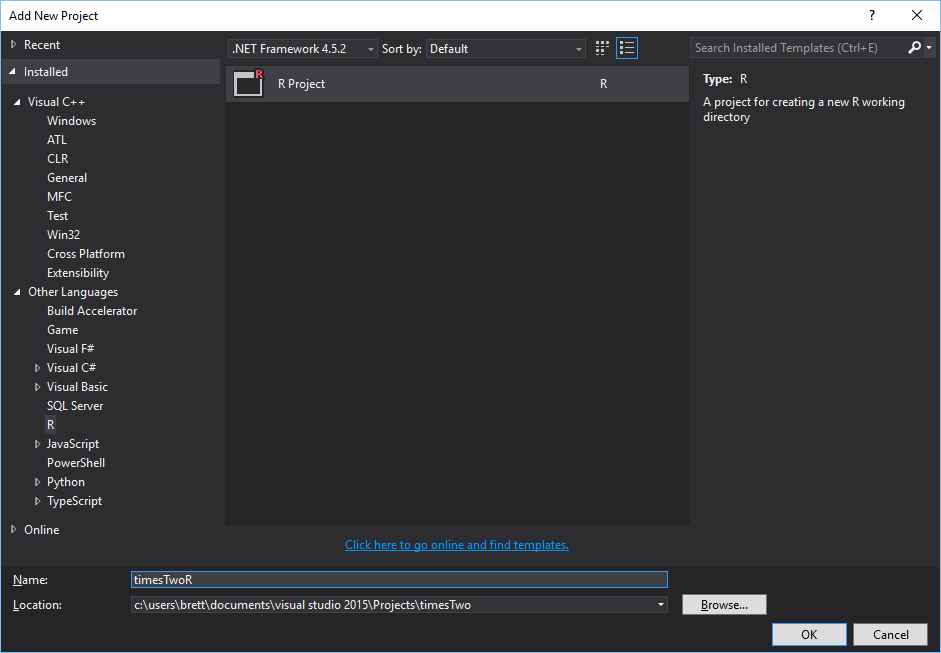
\includegraphics[width=\textwidth,height=0.7\textheight,keepaspectratio]{./timesTwoR.PNG}
}

\end{frame}

\begin{frame}[fragile]{Now run the DLL in R}

\begin{itemize}
\tightlist
\item
  \texttt{dyn.load} loads the .dll into R
\item
  \texttt{.C} calls timesTwo, and passes value\_in and value\_out to the
  function

  \begin{itemize}
  \tightlist
  \item
    \texttt{.C} returns a list, so we define `result' and extract
    `result' from the list
  \end{itemize}
\item
  \texttt{dyn.unload} loads the .dll into R

  \begin{itemize}
  \tightlist
  \item
    you need the unload the dll if you want to rebuild it.
  \end{itemize}
\end{itemize}

\centerline{
  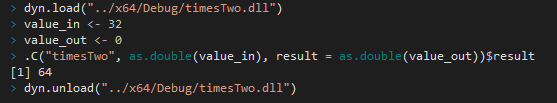
\includegraphics[width=\textwidth,height=0.8\textheight,keepaspectratio]{./DLLinR.PNG}
}

\end{frame}

\begin{frame}[fragile]{Let's change the code for Excel}

\begin{itemize}
\tightlist
\item
  We don't need \texttt{extern\ "C"} anymore
\item
  The function can return a double
\item
  We need to use \texttt{\_\_stdcall}
\item
  Make sure the build matches the Excel version (x64 or x86)
\item
  the .def file remains the same
\end{itemize}

\begin{Shaded}
\begin{Highlighting}[]
\DataTypeTok{double} \NormalTok{__stdcall timesTwo(}\DataTypeTok{double} \NormalTok{*in)}
\NormalTok{\{}
    \DataTypeTok{double} \NormalTok{value = in[}\DecValTok{0}\NormalTok{] * }\FloatTok{2.0}\NormalTok{;}
    \KeywordTok{return} \NormalTok{value;}
\NormalTok{\}}
\end{Highlighting}
\end{Shaded}

\end{frame}

\begin{frame}{In Excel}

\begin{itemize}
\tightlist
\item
  Alt-F11 opens the VBA editor window. Right click on wookbook,
  Insert/Module
\item
  We'll add a declaration for the function in the DLL.
\end{itemize}

\centerline{
  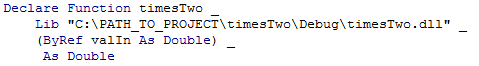
\includegraphics[width=\textwidth,height=0.8\textheight,keepaspectratio]{./vba.png}
}

\begin{itemize}
\tightlist
\item
  Now we can use the function in Excel
\end{itemize}

\centerline{
  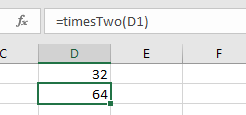
\includegraphics[width=\textwidth,height=0.2\textheight,keepaspectratio]{./inXL.png}
}

\end{frame}

\begin{frame}{Rcpp}

\begin{itemize}
\tightlist
\item
  I wanted to show you how build a DLL in visual studio, because it can
  be useful for more complicated projects
\item
  Often it is easiest to use the Rcpp package instead.
\item
  RCpp makes it easy to pass vectors, matricies, lists, ect, back to R.

  \begin{itemize}
  \tightlist
  \item
    However, there is overhead in doing this.
  \item
    If you are concerned about speed, consider using the simplest
    structure
  \end{itemize}
\end{itemize}

\end{frame}

\begin{frame}[fragile]{Rcpp Example}

\begin{enumerate}
\def\labelenumi{\arabic{enumi}.}
\tightlist
\item
  In RStudio, File / New File / C++ File.
\item
  Enter code in timesTwoRcpp.cpp
\end{enumerate}

\begin{Shaded}
\begin{Highlighting}[]
\OtherTok{#include <Rcpp.h>}
\CommentTok{// [[Rcpp::export]]}
\NormalTok{Rcpp::NumericVector timesTwo(Rcpp::NumericVector x) \{}
  \KeywordTok{return} \NormalTok{x * }\DecValTok{2}\NormalTok{;}
\NormalTok{\}}
\end{Highlighting}
\end{Shaded}

\begin{enumerate}
\def\labelenumi{\arabic{enumi}.}
\setcounter{enumi}{2}
\tightlist
\item
  In R,
\end{enumerate}

\begin{Shaded}
\begin{Highlighting}[]
\KeywordTok{library}\NormalTok{(Rcpp)}
\NormalTok{Rcpp::}\KeywordTok{sourceCpp}\NormalTok{(}\StringTok{"./timesTwoRcpp.cpp"}\NormalTok{)}
\KeywordTok{timesTwo}\NormalTok{(}\KeywordTok{c}\NormalTok{(}\DecValTok{32}\NormalTok{,}\DecValTok{64}\NormalTok{))}
\end{Highlighting}
\end{Shaded}

\begin{verbatim}
## [1]  64 128
\end{verbatim}

\end{frame}

\begin{frame}{Using R's Library}

\begin{itemize}
\tightlist
\item
  Check out R-3.3.0\textbackslash{}include

  \begin{itemize}
  \item
    In that folder there are several header files with functions we can
    use in C/C++
  \item
  \end{itemize}
\end{itemize}

\end{frame}

\begin{frame}{Using R insdie C/C++}

\begin{itemize}
\tightlist
\item
  On linux this is easy and well-documents
\item
  On Windows, it's another story\ldots{}
\item
  I will show you how to do it on Windows,
\item
  Once you know what to do, it is really easy
\end{itemize}

\end{frame}

\begin{frame}[fragile]{Setting up the R API}

\begin{itemize}
\tightlist
\item
  First you need \texttt{pexports} from MinGW.

  \begin{itemize}
  \tightlist
  \item
    We will use \texttt{pexports} to extract information from R.dll to
    create a list of symbols in the DLL
  \item
    Then, we will use this file to generate an import library
  \end{itemize}
\item
  Go to MinGW.org to download the installer. Then, install
  \texttt{pexports}.
\end{itemize}

\centerline{
  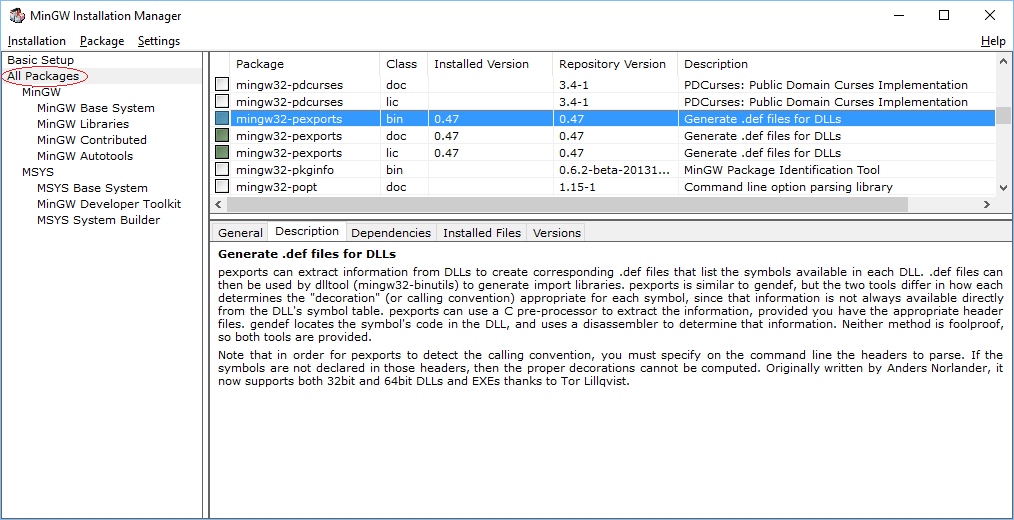
\includegraphics[width=\textwidth,height=0.5\textheight,keepaspectratio]{./pexports.png}
}

\end{frame}

\begin{frame}[fragile]{Setting up the R API}

\begin{enumerate}
\def\labelenumi{\arabic{enumi}.}
\tightlist
\item
  Create the exports definition file from R.dll
\end{enumerate}

\begin{itemize}
\item
  From the command prompt type

\begin{verbatim}
$ cd "C:\Program Files\Microsoft\MRO\R-3.3.0\bin\x64\R.dll"
$ pexports R.dll > R.exp
\end{verbatim}

  \begin{itemize}
  \tightlist
  \item
    Note if pexports is not in your path, you will need to use the full
    path above
  \end{itemize}
\end{itemize}

\begin{enumerate}
\def\labelenumi{\arabic{enumi}.}
\setcounter{enumi}{1}
\item
  Then create the library file using VC++

\begin{verbatim}
$ lib /def:R.exp /out:Rdll.lib /MACHINE:X64
\end{verbatim}

  \begin{itemize}
  \tightlist
  \item
    Now we can use this library in Visual Studio.
  \end{itemize}
\end{enumerate}

\end{frame}

\begin{frame}{Add the path to the R-Version\textbackslash{}include}

\begin{itemize}
\tightlist
\item
  In Visual Studio, right-click the project to open up the property
  pages
\item
  Add the path to the R header files
\end{itemize}

\centerline{
  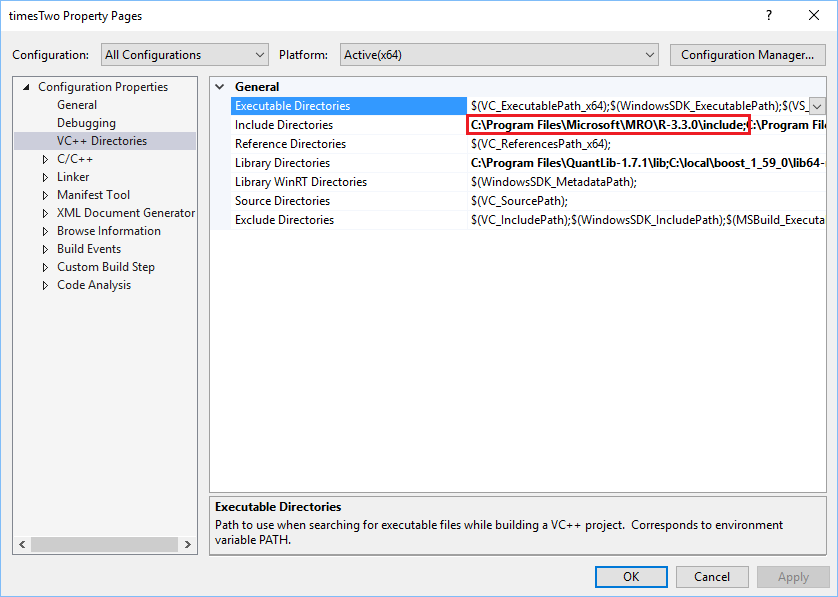
\includegraphics[width=\textwidth,height=0.7\textheight,keepaspectratio]{./inclDir.png}
}

\end{frame}

\begin{frame}{Add the Rdll.lib dependency}

\begin{itemize}
\tightlist
\item
  Property pages/linker/all options
\item
  Add Rdll.lib to the additional dependencies
\item
  Add its path to the additional library Directories
\end{itemize}

\centerline{
  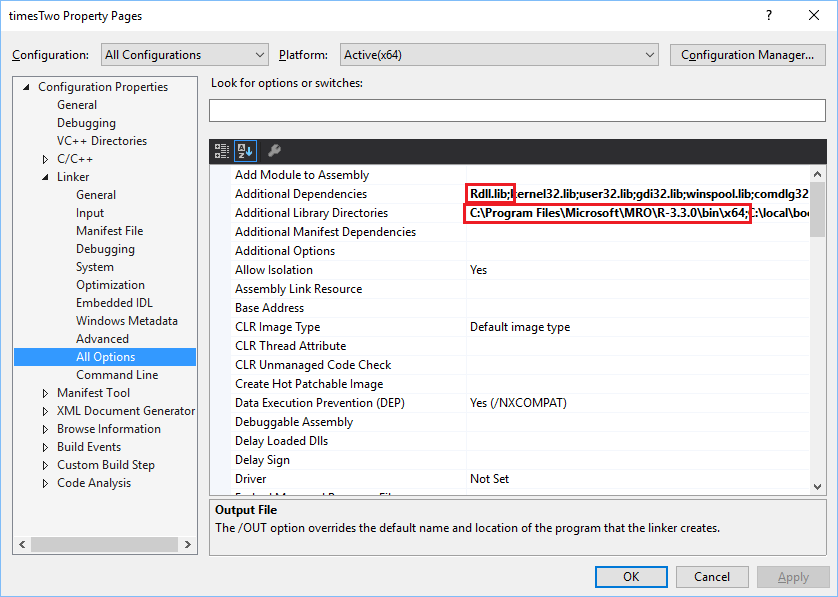
\includegraphics[width=\textwidth,height=0.7\textheight,keepaspectratio]{./linkerOptions.png}
}

\end{frame}

\begin{frame}[fragile]{R's random number generator in C++}

\begin{Shaded}
\begin{Highlighting}[]
\DataTypeTok{extern} \StringTok{"C"} \DataTypeTok{void} \NormalTok{__cdecl randNorm(}\DataTypeTok{double} \NormalTok{*out)}
\NormalTok{\{}
    \NormalTok{GetRNGstate();}
        \NormalTok{out[}\DecValTok{0}\NormalTok{] = norm_rand();}
        \NormalTok{PutRNGstate();}
\NormalTok{\}}
\end{Highlighting}
\end{Shaded}

\end{frame}

\begin{frame}{Resources}

\url{http://adv-r.had.co.nz/C-interface.html}

\end{frame}

\end{document}
